% replace all text with your own text.
% in this template few examples are mention
\chapter{Methodology}
\label{ch:method} % Label for method chapter

\section {Algorithms descriptions}
\textbf {Region-based Convolutional Neural Networks (R-CNN)}: R-CNN is a seminal method for object detection that works by generating region proposals followed by CNN-based feature extraction for each proposal. Initially proposed by  Girshick et al. [8], R-CNN has laid the foundation for subsequent advancements in object detection.


\textbf {Fast R-CNN}: Fast R-CNN [9] improves upon the R-CNN framework by integrating the region proposal mechanism into the network architecture, enabling end-to-end training and faster inference.


\textbf {Faster R-CNN}: Building upon Fast R-CNN, Faster R-CNN [10] introduces a Region Proposal Network (RPN) to efficiently generate region proposals, making the entire detection pipeline faster and more accurate.


\textbf {EfficientDet}: EfficientDet [11] is a scalable and efficient object detection model that achieves state-of-the-art performance by optimizing model architecture and scaling strategies.
You Only Look Once (YOLO) series (YOLOv1-v8):

\clearpage
\textbf{You Only Look Once (YOLO) series (YOLOv1-v8)}:
\begin{figure}[ht]
    \centering
    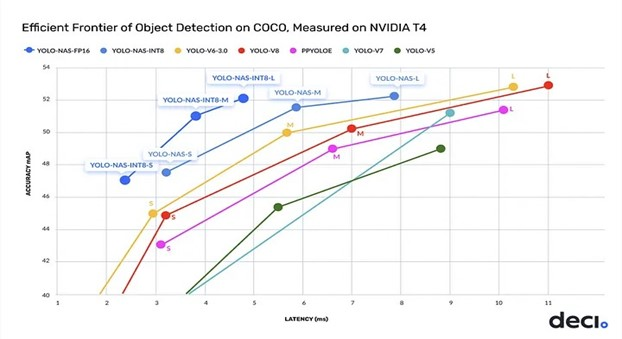
\includegraphics[scale=1.0]{figures/Efficient frointier comparison.jpg}
    \caption{Figure 3.1 Efficient frontier comparison of YOLO models}
    \label{fig:example-01}
\end{figure}

The YOLO series represents a significant advancement in object detection methodology, particularly known for its real-time inference capabilities. YOLOv1 [12] introduced the concept of dividing the input image into a grid and predicting bounding boxes and class probabilities directly from the grid cells. This approach enables YOLO to achieve remarkable speed while maintaining competitive accuracy.

Subsequent iterations of YOLO, including YOLOv2, YOLOv3, YOLOv4, and YOLOv5, have introduced various improvements in terms of speed, accuracy, and model architecture. YOLOv2 [13 ] introduced the concept of anchor boxes for better localization, while YOLOv3 [14] improved upon its predecessor with feature pyramid networks and multi-scale predictions.

YOLOv4 [15] further enhanced the model's performance by incorporating techniques like CSPDarknet53, PANet, and SPP. It achieved state-of-the-art results in terms of both speed and accuracy. YOLOv5 introduced a streamlined architecture and advanced data augmentation techniques, resulting in improved performance and efficiency.

The YOLO series has continued to evolve with the introduction of YOLOv6 and YOLOv7, each bringing novel innovations to the field of object detection. These iterations have focused on optimizing model architectures, training strategies, and inference speed to address various challenges in real-world applications.

YOLO NAS (Neural Architecture Search): YOLO NAS [16] represents a departure from traditional hand-designed architectures by leveraging Neural Architecture Search (NAS) techniques to automatically discover optimal network architectures. By searching through a predefined search space of architectural components, YOLO NAS can tailor the model architecture to specific datasets and tasks, leading to improved performance and efficiency.


\section{Code}:

\begin{lstlisting}[language=Python, caption={Code snippet in \LaTeX ~and  this is a Python code }, label=list:python_code_ex]
import shutil
import os, sys, random
import xml.etree.ElementTree as ET
from glob import glob
import pandas as pd
from shutil import copyfile
import pandas as pd
from sklearn import preprocessing, model_selection
import matplotlib.pyplot as plt
%matplotlib inline
from matplotlib import patches
import numpy as np
import os

labels = sorted(glob('/content/BCCD_Dataset/BCCD/Annotations/*.xml'))
# print(len(labels))
df = []
total = 0
for file in labels:
  prev_filename = file.split('/')[-1].split('.')[0] + '.jpg'
  filename = str(total) + '.jpg'
  row = []
  parsedXML = ET.parse(file)
  for node in parsedXML.getroot().iter('object'):
    blood_cells = node.find('name').text
    xmin = int(node.find('bndbox/xmin').text)
    xmax = int(node.find('bndbox/xmax').text)
    ymin = int(node.find('bndbox/ymin').text)
    ymax = int(node.find('bndbox/ymax').text)

    row = [prev_filename, filename, blood_cells, xmin, xmax, ymin, ymax]
    df.append(row)
  total += 1

data = pd.DataFrame(df, columns=['prev_filename', 'filename', 'cell_type', 'xmin', 'xmax', 'ymin', 'ymax'])

data[['prev_filename','filename', 'cell_type', 'xmin', 'xmax', 'ymin', 'ymax']].to_csv('/content/blood_cell_detection.csv', index=False)

img_width = 640
img_height = 480

def width(df):
  return int(df.xmax - df.xmin)
def height(df):
  return int(df.ymax - df.ymin)
def x_center(df):
  return int(df.xmin + (df.width/2))
def y_center(df):
  return int(df.ymin + (df.height/2))
def w_norm(df):
  return df/img_width
def h_norm(df):
  return df/img_height

df = pd.read_csv('/content/blood_cell_detection.csv')
print(len(df))
le = preprocessing.LabelEncoder()
le.fit(df['cell_type'])
print(le.classes_)
labels = le.transform(df['cell_type'])
df['labels'] = labels

df['width'] = df.apply(width, axis=1)
df['height'] = df.apply(height, axis=1)

df['x_center'] = df.apply(x_center, axis=1)
df['y_center'] = df.apply(y_center, axis=1)

df['x_center_norm'] = df['x_center'].apply(w_norm)
df['width_norm'] = df['width'].apply(w_norm)

df['y_center_norm'] = df['y_center'].apply(h_norm)
df['height_norm'] = df['height'].apply(h_norm)

df.head(30)

df.describe()

df.tail(10)

import cv2
def show_mask(image_name):
  """A function to display image and bounding box"""
  fig = plt.figure(figsize=(6.5, 6.5))
  ax = fig.add_axes([0,0,1,1])
  image = plt.imread('/content/BCCD_Dataset/BCCD/JPEGImages/BloodImage_0000' + image_name)
  plt.imshow(image)

  # ax.imshow(image)

  for _, row in df[df.filename == image_name].iterrows():
        xmin = row.xmin
        xmax = row.xmax
        ymin = row.ymin
        ymax = row.ymax

        width = xmax - xmin
        height = ymax - ymin

        if row.cell_type == 'RBC':
            edgecolor = 'r'
            ax.annotate('RBC', xy=(xmax-40, ymin+20))
        elif row.cell_type == 'WBC':
            edgecolor = 'b'
            ax.annotate('WBC', xy=(xmax-40, ymin+20))
        elif row.cell_type == 'Platelets':
            edgecolor = 'g'
            ax.annotate('Platelets', xy=(xmax-40, ymin+20))

        rect = patches.Rectangle((xmin, ymin), width, height, edgecolor=edgecolor, facecolor='none')
        ax.add_patch(rect)
  plt.title("Blood Cell Types : RBC , WBC , Platelets")
  plt.text(0.5, -0.1, f"Image Width", horizontalalignment='center', verticalalignment='center', transform=plt.gca().transAxes)
  plt.text(-0.1, 0.5, f"Image Height", horizontalalignment='center', verticalalignment='center', rotation=90, transform=plt.gca().transAxes)
 plt.show()

show_mask('1.jpg')
show_mask('2.jpg')
show_mask('3.jpg')

Dataset Distribution

from sklearn.model_selection import train_test_split
df_train_temp, df_valid = train_test_split(df, test_size=0.10, random_state=42, shuffle=True, stratify=df['cell_type'])
df_train, df_test = train_test_split(df_train_temp, test_size=0.075, random_state=42, shuffle=True, stratify=df_train_temp['cell_type'])

Data Visualization

"""Plotting of total instances of RBC ,WBC ,Platelets in Train,Validation an Test Dataset"""
plt.subplot(1, 3, 2)
plt.bar(valid_class_counts.index, valid_class_counts.values)
plt.title('Validation Set Class Distribution')
plt.xlabel('Classes')
plt.ylabel('Instance Count')

plt.subplot(1, 3, 3)
plt.bar(test_class_counts.index, test_class_counts.values)
plt.title('Test Set Class Distribution')
plt.xlabel('Classes')
plt.ylabel('Instance Count')

plt.tight_layout()
plt.show()

""Plotting total count of images in train, validation, and test sets"""
plt.figure(figsize=(10, 5))

labels = ['Train', 'Validation', 'Test']
values = [train_total_images, valid_total_images, test_total_images]

plt.bar(labels, values, color=['orange', 'blue', 'red'])
plt.title('Total Count of Images in Train, Validation, and Test Sets')
plt.xlabel('Datasets')
plt.ylabel('Image Count')
plt.show()

\end{lstlisting}

\section{Implementation}
\textbf{YOLO NAS Model Selection}: YOLO NAS model architecture was used for object detection experiments. Consider YOLO NAS-S, YOLO NAS-M, and YOLO NAS-L variants.
\textbf{Training Configuration}: Configured the training parameters including the number of epochs (50-100), batch size (8,16,32), optimizer (e.g., Adam), learning rate schedule (e.g., cosine annealing with warm-up), loss function (e.g., YOLO loss), and any additional metrics for evaluation (e.g., mAP, precision, recall).

\textbf{You Only Look Once (YOLO) series (YOLOv1-v8)}:
\begin{figure}[ht]
    \centering
    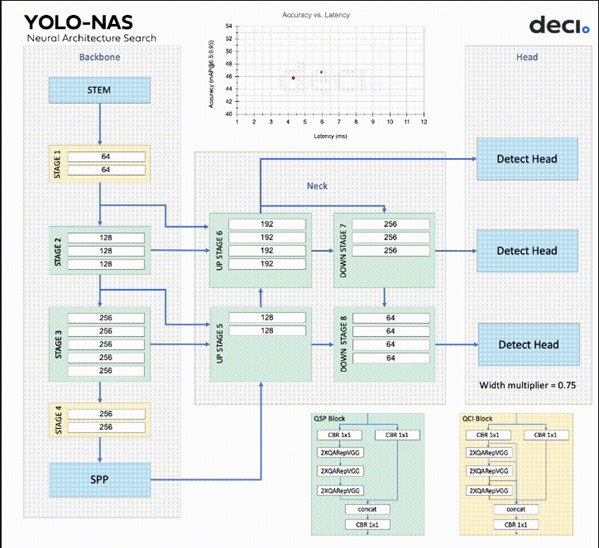
\includegraphics[scale=1.0]{figures/YOLO-NAS Neural Architecture Search.jpg}
    \caption{Figure 3.2 : YOLO-NAS Neural Architecture Search}
    \label{fig:example-01}
\end{figure}


\textbf{Dataset Preparation}: The dataset was prepared for training, validation , and testing . This includes data preprocessing steps such as annotation extraction, data augmentation, and splitting the dataset into training (80%), validation (10%), and test sets(10%).
\textbf{Inference}: Set up the inference pipeline for performing object detection on new images using the trained YOLO NAS models.
\textbf{Evaluation}: Implement the evaluation pipeline to calculate performance metrics such as mAP@0.50:0.95, precision@0.50:0.95, and recall@0.50:0.95 on the test dataset.

\section{Experiments Design}:
\textbf{Model Evaluation}: Evaluate YOLO NAS models (YOLO NAS-S, YOLO NAS-M, YOLO NAS-L) on the selected metrics (mAP@0.50:0.95, precision, recall) for different configurations.
\textbf{Hyperparameter Tuning}: Experiment with different hyperparameters such as input image sizes, number of epochs, and quantization levels (8-bit, 16-bit, 32-bit).
\textbf{Input Image Sizes}: Experiment with different input image sizes to observe their impact on model performance and inference speed.
\textbf{Quantization Levels}: Experiment with different quantization levels (8-bit, 16-bit, 32-bit) to analyze the trade-off between model accuracy and computational efficiency.
\textbf{Epochs}: Train the models for different numbers of epochs (e.g., 50, 75, 100) to observe the convergence behavior and model performance over time.
\textbf{Comparison with YOLO-S, YOLO-M, YOLO-L}: Compare the performance of YOLO NAS models with standard YOLO variants (YOLO-S, YOLO-M, YOLO-L) on the specified metrics.

\section{Experimental Procedure}:
Initialize the selected YOLO NAS model architecture.
Train the model using the training dataset with the specified configurations (epochs, batch size, etc.). Validate the trained model on the validation dataset to monitor performance metrics. Fine-tune the model if necessary based on validation results.Evaluate the final trained model on the test dataset to report the performance metrics (mAP@0.50:0.95, precision, recall).
Repeat the experiments for different configurations and variations.

\section{Results Analysis}:
Analyze the experimental results to identify the optimal YOLO NAS model configuration based on the specified metrics.

Compare the performance of YOLO NAS models with standard YOLO variants and observe any differences in accuracy, speed, and efficiency.

Discuss the impact of hyperparameters (input image sizes, epochs, quantization levels) on model performance and computational efficiency.

Interpret the results to draw conclusions and insights regarding the effectiveness of YOLO NAS for object detection tasks.
